\documentclass[a4paper,11pt]{scrartcl}
\usepackage{graphicx}
\usepackage{amsfonts}
\usepackage{amsmath}
\usepackage{amssymb}
\usepackage{mathtools}
\usepackage{bm}
\usepackage{amsbsy}
\usepackage{algorithmic}
\usepackage{algorithm}
\usepackage{listings}
\usepackage{tikz}
\usepackage{stackrel}
\usepackage{url}
\usepackage{xspace}
%\usepackage{cite}
\usepackage{enumerate}
\usepackage{enumitem}
\usepackage[pagewise]{lineno}
\usepackage{ulem}             %% strikeout text
\usepackage{color}            %% color

%Packages for table
\usepackage{tabularx, booktabs}
\usepackage{diagbox}
\usepackage[tableposition = top]{caption}
\usepackage{booktabs}
\usepackage{siunitx}
\usepackage{stmaryrd}
\usepackage{pgfplots}
\newcommand*\mc[1]{\multicolumn{1}{c}{#1}}

% font
\usepackage[T1]{fontenc}
\usepackage[ansinew]{inputenc}
\usepackage{lmodern}

% pdf
\usepackage{ifpdf}\ifpdf\usepackage{epstopdf}\fi

% geometry
\usepackage[letterpaper,centering]{geometry}
\geometry{textheight=8.5in,textwidth=7in}

%%%%%%%%%%%%%%%%%%%%%%%%%%%%%%%%%%%%%%%%

% commandes persos
\newcommand{\Ac}{{\mathscr A}}
\newcommand{\Rb}{{\mathbb{R}}}
\newcommand{\Bc}{{\mathcal{B}}}
\newcommand{\Dc}{{\mathcal{D}}}
\newcommand{\Oc}{{\mathcal{O}}}
\newcommand{\Var}{{\mathbb{V}}}
\newcommand{\Cov}{{\text{Cov}}}
\newcommand{\Pb}{{\mathbb{P}}}
\newcommand{\Esp}{{\mathbb{E}}}
\newcommand{\dd}{{\text{d}}}


% \renewcommand{\span}{{\text{span}}}

% couleur style alert

\newcommand{\alert}[1]{\textcolor{red}{#1}}

% SPAN
\DeclareMathOperator{\spann}{span}

%indicatrice avec commande \one
\DeclareMathAlphabet{\mathonebb}{U}{bbold}{m}{n}
\newcommand{\one}{\ensuremath{\mathonebb{1}}}

\begingroup
%\usepackage[math]{anttor}
\makeatletter
\renewcommand{\rmdefault}{antt}
  \DeclareMathVersion{antt}
    \DeclareMathVersion{anttbold}
    \SetSymbolFont{operators}{antt}{OT1}{\rmdefault m}{m}{n}
    \SetSymbolFont{letters}{antt}{OML}{\rmdefault} {m}{it}
    \SetSymbolFont{symbols}{antt}{OMS}{\rmdefault}{m}{n}
    \SetSymbolFont{largesymbols}{antt}{OMX}{\rmdefault}{m}{n}
    \SetSymbolFont{operators}{anttbold}{OT1}{\rmdefault m} {b}{n}
    \SetSymbolFont{letters}  {anttbold}{OML}{\rmdefault} {b}{it}
    \SetSymbolFont{symbols}  {anttbold}{OMS}{\rmdefault}{b}{n}
    \SetSymbolFont{largesymbols}{anttbold}{OMX}{\rmdefault}{b}{n}
  %  \egroup
    \SetMathAlphabet{\mathbf}{antt}{OT1}{\rmdefault}{bx}{n}
    \SetMathAlphabet{\mathsf}{antt}{OT1}{\rmdefault}{m}{n}
    \SetMathAlphabet{\mathit}{antt}{OT1}{\rmdefault}{m}{it}
    \SetMathAlphabet{\mathtt}{antt}{OT1}{\rmdefault}{m}{n}
    \SetMathAlphabet\mathsf{anttbold}{OT1}{\rmdefault}{bx}{n}
    \SetMathAlphabet\mathit{anttbold}{OT1}{\rmdefault}{bx}{it}
\gdef\newgamma{\mbox{\mathversion{antt}$\gamma$}}
\endgroup
\makeatother

% structures habituelles: thm, prop, preuve...
\newtheorem{theorem}{Theorem}[section]
\newtheorem{acknowledgement}[theorem]{Acknowledgement}
%\newtheorem{algorithm}{Algorithm}
%\newtheorem{axiom}[theorem]{Axiom}
%\newtheorem{case}[theorem]{Case}
%\newtheorem{claim}[theorem]{Claim}
\newtheorem{conclusion}[theorem]{Conclusion}
\newtheorem{condition}[theorem]{Condition}
\newtheorem{conjecture}[theorem]{Conjecture}
\newtheorem{corollary}[theorem]{Corollary}
\newtheorem{assumption}[theorem]{Assumption}
\newtheorem{criterion}[theorem]{Criterion}
\newtheorem{definition}[theorem]{Definition}
\newtheorem{example}[theorem]{Example}
\newtheorem{exercise}[theorem]{Exercise}
\newtheorem{lemma}[theorem]{Lemma}
\newtheorem{notation}[theorem]{Notation}
\newtheorem{problem}[theorem]{Problem}
\newtheorem{proposition}[theorem]{Proposition}
\newtheorem{remark}[theorem]{Remark}
\newtheorem{solution}[theorem]{Solution}
\newtheorem{summary}[theorem]{Summary}
\newtheorem{rem}[theorem]{Remark}
\newtheorem{property}[theorem]{Property}

%%%%%%%%%%%%%%%%%%%%%%%%%%%%%%
%% Raccourci %%
\newcommand{\R}{\mathbb{R}}
\newcommand{\N}{\mathbb{N}}

\newcommand{\eq}[1]{\begin{equation} #1 \end{equation}}
\newcommand{\eqs}[1]{\begin{align} #1 \end{align}}
\newcommand{\inner}[2]{\left\langle #1, #2\right\rangle}

\DeclareOldFontCommand{\bf}{\normalfont\bfseries}{\mathbf}
\DeclareOldFontCommand{\rm}{\normalfont\rmfamily}{\mathrm}

\setlength{\parindent}{0pt}
\setlength{\parskip}{11pt}

\graphicspath{{fig/}}

\begin{document}


% title
\begin{center}
{\Large
{\rule{\linewidth}{2pt}}\\[0.5cm]
{\bf Model Reduction for Nonlinear Partial Differential Equations}\\
\normalsize Tiangang Cui \\ \today\\[0.25cm]
{\rule{\linewidth}{2pt}}
}
\end{center}

This document is outdated. The assembly of the stiffness matrix needs to be updated. 


\section{Introduction}


Many mathematical models in continuum mechanics demonstrate nonlinear behaviour. Common examples can be seen in non-Newtonian fluids where viscous stresses of fluids nonlinearly dependent on shear rates, in finite elasticity models where stress tensors can be nonlinear functions of the deformation gradient, and in in porous media flows where relative permeabilities and capillary pressures are nonlinear functions of flow pressure and saturation.
%
Numerical methods such as finite element and finite volume have demonstrated tremendous success in solving the governing partial differential equations of these nonlinear systems, whereas little progress has been made on constructing projection-based reduced order models for these nonlinear PDEs.

Considering the steady state solution, a common feature shared between these nonlinear models is that the resulting discretised PDE takes the form of
\begin{equation}
A(\theta, u) u + f(\theta, u) = 0,
\end{equation}
where $A$ is the operator, $u$ is the model state, and $\theta$ is the input parameter.
%
Here we want to design and analyse various projection-based model reduction strategies for this type of PDEs.

We first investigate the p-Poisson problem, and then apply strategies developed to the non-Newtonian Stoke's flow.

\section{$p$-Poisson problem}

In a domain $\Omega \subset \real^d$ with spatial dimension $d = 2$ or $d = 3$, we consider the p-Poisson equation
\eq{ - \nabla \cdot \left( \eta\left(u\right) \nabla u \right) - f = 0 ,}
with diffusivity
\eq{ \eta(u) = ( 2 \gamma(u) + \epsilon )^{\frac{p-2}{2}} ,\quad \gamma(u) = \frac12 |\nabla u|^2, }
which is a nonlinear function of the potential.
%
Here $\epsilon > 0$ is a regularisation term to avoid singular ($p < 2$) or degenerate ($p > 2$) solutions at $\nabla u = 0$.

%We first consider a two dimensional test case on a unit square, e.g., $\Omega = [0, 1]^2$, with a mixed boundary condition: zero Neumann boundary conditions on the left and right, zero Dirichlet boundary condition on the top, and Robin boundary condition on the bottom. This way, the system of governing equations becomes:
%\eqs{
%- \nabla \cdot ( \eta(u ) \nabla u ) - f = 0 \quad & {\rm on} \quad \Omega , \\
%\eta(u) \nabla u \cdot n = 0 \quad & {\rm on} \quad \partial \Omega_{\rm l} \cup \partial \Omega_{\rm r}, \\
%u = 0 \quad & {\rm on} \quad \partial \Omega_{\rm t}, \\
%\eta(u) \nabla u \cdot n + \beta u = 0 \quad & {\rm on} \quad \partial \Omega_{\rm b} .
%}
We first consider a two dimensional test case on a unit square, e.g., $\Omega = [0, 1]^2$, with a mixed boundary condition: zero Neumann boundary conditions on the left, right and top, and Robin boundary condition on the bottom. This way, the system of governing equations becomes:
\eqs{
- \nabla \cdot ( \eta(u ) \nabla u ) - f = 0 \quad & {\rm on} \quad \Omega , \\
\eta(u) \nabla u \cdot n + \beta u = 0 \quad & {\rm on} \quad \partial \Omega_{\rm b} , \\
\eta(u) \nabla u \cdot n = 0 \quad & {\rm on} \quad \partial \Omega \setminus \partial \Omega_{\rm b}.
}

\subsection{Weak form}
%
%We aim to find a weak form solution $u \in H^1(\Omega)$ such that
%\eq{ - \int_{\Omega}  v \nabla \cdot ( \eta(u ) \nabla u) - \int_{\Omega} vf  +  \rho \int_{\partial \Omega_{\rm t}} vu = 0 ,}
%for all test functions $v \in H^1(\Omega)$. Here $\alpha > 0$ is a penalty term to enforce Dirichlet boundary condition at the top. {\color{red} is this right? and how to choose the penalty?}
%%
%Applying Green's identity, the above weak form implies
%\eq{ \int_{\Omega} \nabla v \cdot \eta(u) \nabla u - \int_{\partial\Omega} (\eta(u) \nabla u  \cdot n ) v  - \int_{\Omega} vf +  \rho \int_{\partial \Omega_{\rm t}} vu = 0 }


We aim to find a weak form solution $u \in H^1(\Omega)$ such that
\eq{ - \int_{\Omega}  \nabla \cdot ( \eta(u ) \nabla u) v - \int_{\Omega} f v  = 0 ,}
for all test functions $v \in H^1(\Omega)$.
%
Applying Green's identity and boundary conditions, the above weak form implies
\eq{ \int_{\Omega} (\eta(u) \nabla u) \cdot \nabla v+ \int_{\partial\Omega_{\rm b}} \beta uv  - \int_{\Omega} fv = 0 . \label{eq:pp_weak}}
%
The solution of this weak form can be obtained using some root-finding algorithms such as the Newton-Raphson. Alternatively, using the variational approach, we can naturally interpret the above weak form as the first order necessary condition of an energy minimisation problem.

Define the energy functional
\eq{ \mathcal{E}(u) =  \int_{\Omega} \tfrac{1}{p}  (2\gamma(u) + \epsilon)^{\frac{p}{2}}  .\label{eq:energy}}
%
Since the directional derivative of $\gamma(u)$ along a function $v$ is $ \gamma'(u)[v] = \nabla u \cdot \nabla v$,
%
the variation of $\mathcal{E}(u)$ along a function $v$ takes the form
\eqs{ \mathcal{E}^\prime(u)[v]  & = \int_{\Omega}  (2\gamma(u) + \epsilon)^{\frac{p-2}{2}} \nabla u \cdot \nabla v\\
 & = \int_{\Omega}  \eta(u) \nabla u \cdot \nabla v. }
%
Similarly, given the directional derivative of $\eta(u)$ along a function $w$,
\eqs{
\eta^\prime(u)[w] & = (p-2) \frac{\eta(u)}{2\gamma(u) + \epsilon} \gamma'(u)[w] \nonumber \\
& = (p-2) \frac{\eta(u)}{2\gamma(u) + \epsilon} \nabla u \cdot \nabla w,
}
%
the variation of $\mathcal{E}^\prime(u)[v]$ along a function $w$ takes the form
\eqs{ \mathcal{E}^{\prime\prime}(u)[v]\{w\} & = \int_{\Omega} \eta'(u)[w] \nabla u \cdot \nabla v + \int_{\Omega}  \eta(u) \nabla w \cdot \nabla v \nonumber \\
& = (p-2) \int_{\Omega} \frac{\eta(u)}{2\gamma(u) + \epsilon} (\nabla v \cdot \nabla u)( \nabla u \cdot \nabla w )+ \int_{\Omega} \eta(u) \nabla v \cdot \nabla w .}
Defining the tensor
\eq{
A(u) = \eta(u) \left(I + (p-2)\frac{\nabla u \otimes \nabla u}{2\gamma(u) + \epsilon} \right),
}
and the vector
\eq{
b(u) = \left( 2\gamma(u) + \epsilon \right)^{\frac{p}{4}-1} \nabla u,
}
such that
\eq{
 b(u) \otimes b(u) = \frac{\eta(u)}{2\gamma(u) + \epsilon} \nabla u \otimes \nabla u,
}
the above equation can be rewritten as
\eq{\mathcal{E}^{\prime\prime}(u)[v]\{w\} = \int_{\Omega} \nabla v : A(u) : \nabla w ,}
or
\eq{\mathcal{E}^{\prime\prime}(u)[v]\{w\} = (p-2) \int_{\Omega} \left(\nabla v \cdot b(u)\right) \left( \nabla w\cdot b(u) \right) + \int_{\Omega} \eta(u) \nabla v \cdot \nabla w .}


This way, the objective function of the minimisation problem corresponding to the solution of \eqref{eq:pp_weak} is
\eq{ \mathcal{J}(u) = \int_{\Omega} \tfrac{1}{p}  (2\gamma(u) + \epsilon)^{\frac{p}{2}} + \frac12\int_{\partial\Omega_{\rm b}} \beta u^2  - \int_{\Omega} fu. }
%
Its variation along a function $v$,
\eq{ \mathcal{J}^\prime(u)[v] = \int_{\Omega} \eta(u) \nabla u \cdot \nabla v + \int_{\partial\Omega_{\rm b}} \beta uv  - \int_{\Omega} fv ,}
is simply the left hand side of equation \eqref{eq:pp_weak}, and its second order variation along function $w$ for given $u$ and $v$ is
\eq{\mathcal{J}^{\prime\prime}(u)[v]\{w\}  = (p-2) \int_{\Omega} \left(\nabla v \cdot b(u)\right) \left( \nabla w\cdot b(u) \right) + \int_{\Omega} \eta(u) \nabla v \cdot \nabla w  + \int_{\partial\Omega_{\rm b}} \beta vw .}
%
Given $\mathcal{J}(u)$, $\mathcal{J}^\prime(u)[v]$ and $\mathcal{J}^{\prime\prime}(u)[v]\{w\}$, sophisticated nonlinear optimisation methods such as inexact Newton, subspace trust region and linear search can be used to find a solution of the weak form \eqref{eq:pp_weak}.

\subsection{Analytical solution}

We use a reference solution
\eq{u(x_1, x_2) = ( 1 - \cos(2 \pi x_1) ) \sin(1.25 \pi x_2 + 0.25 \pi ),}
which satisfies the no flux boundary conditions on left, right and top boundaries, to manufacture a forcing term and a boundary function $\beta$.
%
Figure \ref{fig:pp_ref} shows the reference solution, and Figures \ref{fig:pp_ref} and \ref{fig:pp_bnd} show the manufactured forcing and $\beta$ function that controls Robin boundary condition at the bottom.


\begin{figure}
\centerline{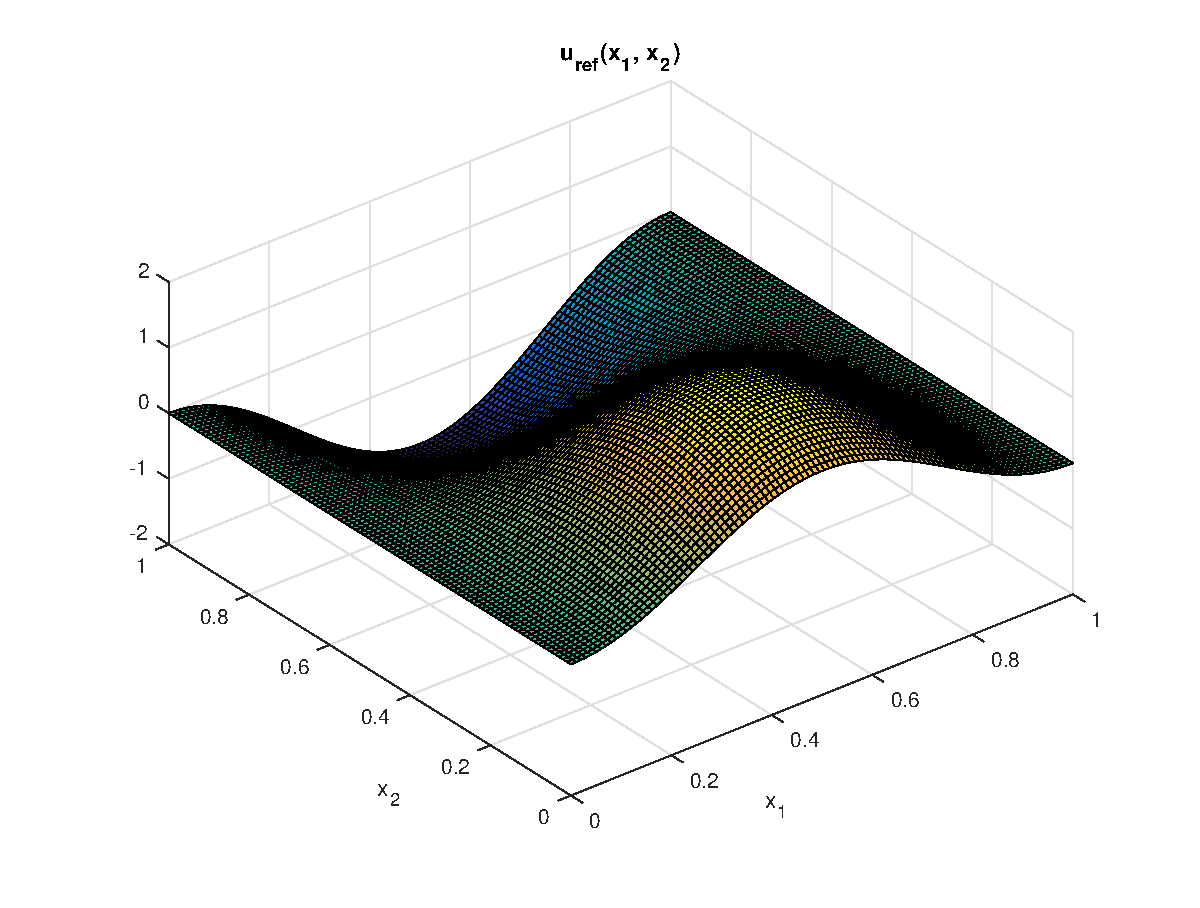
\includegraphics[width=0.8\textwidth]{ref_state.eps}}
\centerline{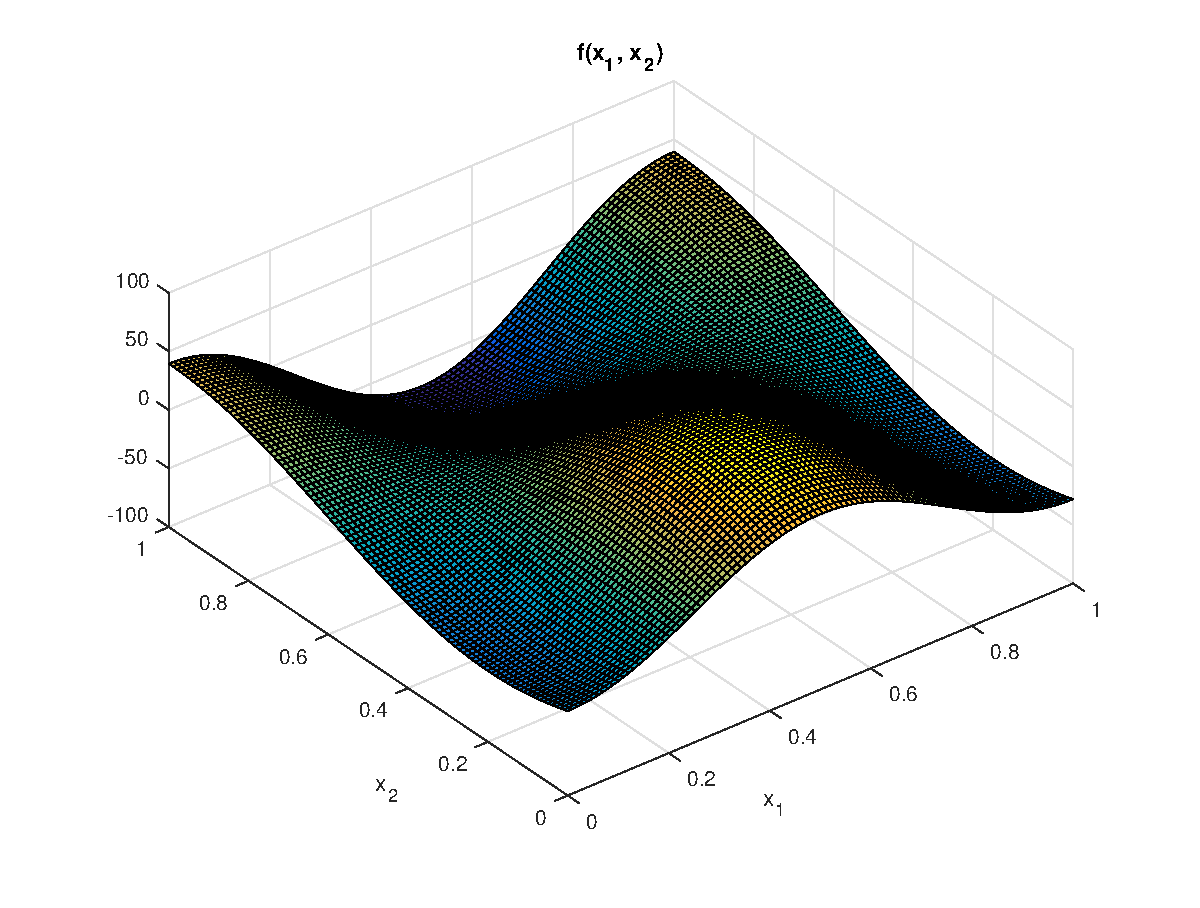
\includegraphics[width=0.8\textwidth]{ref_forcing.eps}}
\caption{Reference solution and forcing of the $p$-Poisson problem. }
\label{fig:pp_ref}
\end{figure}

\begin{figure}
\centerline{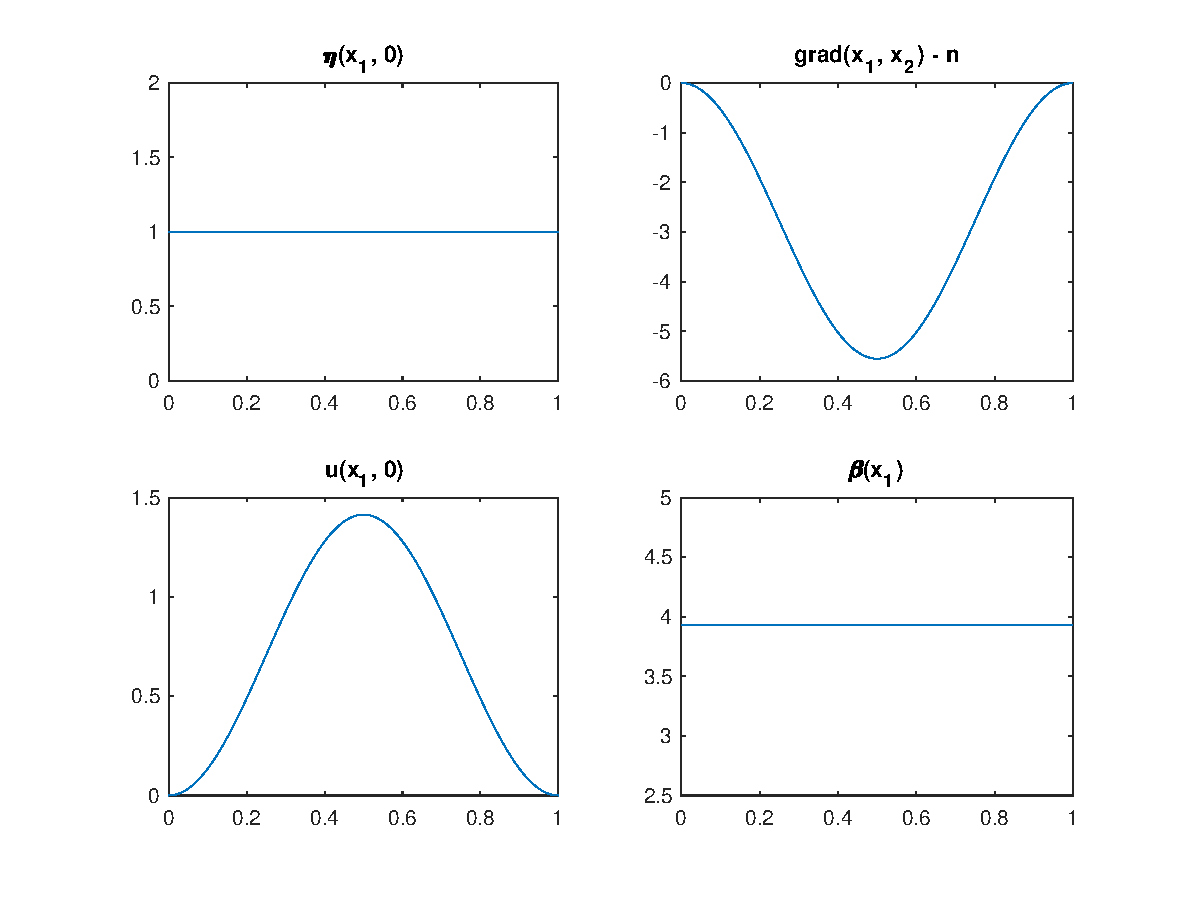
\includegraphics[width=0.8\textwidth]{ref_boundary_p2.eps}}
\caption{Boundary condition at $x_2 = 0$ that generates the reference solution for $p=2$. }
\label{fig:pp_bnd}
\end{figure}

We use the MATLAB symbolic package to generate symbolic functions of the state, forcing, and $\beta$ for validating the FEM implementation.
%
This is implemented in ``ref\_soln2d.m'', using the following lines key codes:

\begin{verbatim}
syms x1 x2

% state_func(x1, x2) = ( 1 - cos(2*pi*x1) ) * sin( 0.25*pi*(1-x2) );
state_func(x1, x2) = ( 1 - cos(2*pi*x1) ) * sin(1.25*pi*x2 + 0.25*pi );

ds_x1(x1, x2) = diff(state_func, x1);
ds_x2(x1, x2) = diff(state_func, x2);

% eta
grad_s_l2n(x1, x2) = ds_x1(x1, x2)^2 + ds_x2(x1, x2)^2;
eta_func(x1, x2) = (grad_s_l2n(x1, x2) + epsilon)^(p_rate/2-1);

% forcing
forcing_func(x1, x2) = - (diff(eta_func*ds_x1, x1) + ...
    diff(eta_func*ds_x2, x2));

% robin at bottom boundary
grad_s_dot_n(x1) = -ds_x2(x1, 0);
beta_func(x1) = -eta_func(x1,0)*grad_s_dot_n(x1)/state_func(x1,0);
\end{verbatim}


\subsection{Finite element implementation}

\subsubsection{Simplex element}
\def\arraystretch{1.5}
%
\newcommand{\centerrow}[1]{\smash{\raisebox{.6\normalbaselineskip}{#1}}}
%
\newcommand{\vertices}{\left[ \begin{array}{l|l|l} x^{(1)}_1 & x^{(2)}_1 & x^{(3)}_1 \\ x^{(1)}_2 & x^{(2)}_2 & x^{(3)}_2 \\ 1 & 1 & 1 \end{array} \right]}
%
\newcommand{\bcoord}{\left[ \begin{array}{l} \lambda_1 \\ \lambda_2 \\ 1 - (\lambda_1 + \lambda_2) \end{array} \right]}
%
\newcommand{\ax}{\left[ \begin{array}{l} x_1 \\ x_2 \\ 1 \end{array} \right]}
%

The local finite element basis function is based on the barycentric coordinate. In two spatial dimension, we have barycentric coordinates $(\lambda_1, \lambda_2)$ and let $\lambda_3 = 1 - (\lambda_1 + \lambda_2)$ as shown in Figure \ref{fig:bary}.
%
The coordinates transformation between Cartesian and barycentric coordinates are
\eq{
\ax = \vertices \bcoord,
}
and
\eq{
\bcoord = \vertices^{-1} \ax.
}

\begin{figure}[h]
\pgfplotsset{width=0.45\textwidth}
\begin{center}
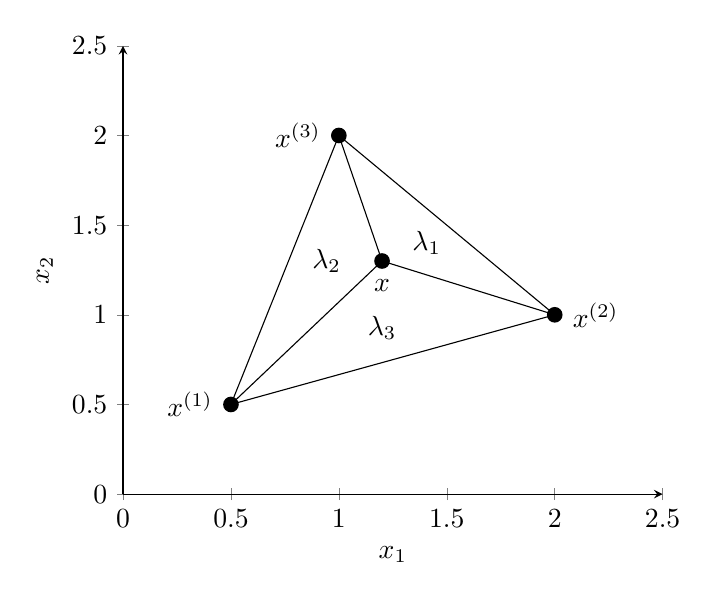
\begin{tikzpicture}

\begin{axis}[
    axis lines = left,
    xlabel = $x_1$,
    ylabel = $x_2$,
    xmin=0, xmax=2.5,
    ymin=0, ymax=2.5,
]

%
\addplot[color=black,mark=circle]
    coordinates {
    (0.5,0.5)(2,1)(1,2)(0.5,0.5)
    };
\addplot[color=black,mark=circle]
    coordinates {
    (0.5,0.5)(1.2,1.3)
    };
\addplot[color=black,mark=circle]
    coordinates {
    (2,1)(1.2,1.3)
    };
\addplot[color=black,mark=circle]
    coordinates {
    (1,2)(1.2,1.3)
    };

\node[label={180:{$x^{(1)}$}},circle,fill,inner sep=2pt] at (axis cs:0.5,0.5) {};
\node[label={  0:{$x^{(2)}$}},circle,fill,inner sep=2pt] at (axis cs:2,1) {};
\node[label={180:{$x^{(3)}$}},circle,fill,inner sep=2pt] at (axis cs:1,2) {};
\node[label={270:{$x$}},circle,fill,inner sep=2pt] at (axis cs:1.2,1.3) {};
%
\node[label={0:{$\lambda_1$}}] at (axis cs:1.25,1.4) {};
\node[label={180:{$\lambda_2$}}] at (axis cs:1.1,1.3) {};
\node[label={270:{$\lambda_3$}}] at (axis cs:1.2,1.1) {};

\end{axis}
\end{tikzpicture}
%
\begin{tikzpicture}
\begin{axis}[
    axis lines = left,
    xlabel = $\lambda_1$,
    ylabel = $\lambda_2$,
    xmin=-0.4, xmax=1.4,
    ymin=-0.4, ymax=1.4,
]

\addplot[
    color=black,
    mark=circle,
    ]
    coordinates {
    (0,0)(1,0)(0,1)(0,0)
    };

\node[label={180:{$x^{(3)}$}},circle,fill,inner sep=2pt] at (axis cs:0,0) {};
\node[label={  0:{$x^{(1)}$}},circle,fill,inner sep=2pt] at (axis cs:1,0) {};
\node[label={180:{$x^{(2)}$}},circle,fill,inner sep=2pt] at (axis cs:0,1) {};

\end{axis}
\end{tikzpicture}
\end{center}
\caption{Barycentric coordinate}
\label{fig:bary}
\end{figure}

Let $x = [x_1, \ldots, x_d]^\top$ and $\lambda = [\lambda_1, \ldots, \lambda_d]^\top$ be the Cartesian and barycentric coordinates in $\R^d$.
%
%In our implementation, the cartesian  coordinates of the element vertices is organised as
%\eq{
%V_e = \left[ \begin{array}{c|c|c} x^{(1)} & \cdots &  x^{(d+1)} \\ 1 & \cdots & 1 \end{array} \right]^\top,
%}
%and hence the transformation pair becomes
%\eqs{
%\left[ \begin{array}{l|l} x^\top & 1 \end{array} \right] & = \left[ \begin{array}{l|l} \lambda^\top & 1 - \sum_{i}\lambda_i \end{array} \right] V_e , \\
%\left[ \begin{array}{l|l} \lambda^\top & 1 - \sum_{i}\lambda_i \end{array} \right] & = \left[ \begin{array}{l|l} x^\top & 1 \end{array} \right] V_e^{-1}.
%}
%%
%This leads to the following transformation pair between $x$ and $\lambda$:
%
For $e$-th element, the affine transformation $x = \varphi_e (\lambda)$ from the barycentric coordinate to the Cartesian coordinate can be defined by
\eq{
x =  T^{(e)}_{\rm ref} \lambda + x^{(e)}_{\rm ref} \label{eq:l2g} ,
}
where $T^{(e)}_{\rm ref} = \left[ x^{(1)} \vert \cdots \vert  x^{(d)} \right] -  x^{(d+1)} {\bf 1}_d^\top$ and $x^{(e)}_{\rm ref} = x^{(d+1)}$ are reference transformation matrix and reference point, respectively.

\subsubsection{Local basis functions}

We use the multi-index notation to generate a set of polynomial functions up to order $p$. This leads to a multi-index matrix $\alpha \in \N^{n_b \times d}$, where the number of rows $n_b$ should equal to the number of nodal points used to define the local basis functions.
%
The linear combination of this set of polynomials can be used to define a set of Lagrange  basis functions
\eq{
\phi_i(\lambda) = \sum_{j=1}^{n_b} A_{ij} \prod_{k=1}^{d} \lambda_k^{\alpha_{jk}}, \quad 1 \leq i \leq n_b,
}
where $A\in \N^{n_b \times n_b}$ is the coefficient matrix.
%
Given a set of nodal points $\{\lambda^{(j)}\}$ where $1 \leq j \leq n_b$, the property of Lagrange function
\eq{
\phi_i(\lambda^{(j)}) = \delta_{ij},
}
is then used to evaluate the coefficient of the Lagrange basis functions $A_{ij}$.
%
The derivative of the basis function is
\eq{
\frac{\partial \phi_i(\lambda)}{\partial \lambda_l} = \sum_{j=1}^{n_b} A_{ij} \alpha_{jl} \lambda_l^{\alpha_{jl} - 1} \prod_{k \neq l}^{d} \lambda_k^{\alpha_{jk}}.
}

\subsubsection{FEM implementation}

The above definition of local basis function defines the following set of global finite element basis functions,
\eq{
\psi_i(x) =  \sum_{e \sim x^{(i)}} \sum_{j=1}^{n_b} \phi_j( \varphi_e^{-1}(x^{(i)}) ) \, \phi_j( \varphi_e^{-1}(x) ) \label{eq:global}
}
where the notation $e \sim x^{(i)}$ denotes all the elements connect to a node $x^{(i)}$.
%
This above global function is the summation of all the local basis functions that have value one at node $x^{(i)}$, which is enforced by $\phi_j( \varphi_e^{-1}(x^{(i)}) )$ in \eqref{eq:global}.
%
We note that the global basis function also satisfies the property of Lagrange function.
%
This way, a function $u$ can be approximated by either a linear combination of global basis functions
\eq{
u(x) \approx u^h(x) := \sum_{i=1}^{N} \psi_i(x) u_i,
}
where $u_i = u(x^{(i)})$, or a linear combination of local basis functions
\eq{
u^h(x) = \sum_{e} \sum_{j=1}^{n_b} \phi_j( \varphi_e^{-1}(x) ) u_j = \sum_{e} \sum_{j=1}^{n_b} \phi_j( \lambda ) u_j,
}
where $u_j = u(\varphi_e(\lambda^{(j)}))$.
%
An integral over the original domain $\Omega$ can be written as the summation of integrals over each of local element, i.e.,
\eq{
\int_{\Omega} f(x) dx = \sum_{e} \int_e f(x) dx.
}
This way, the integration problem can be broken into element-wise integrations.
%
In implementing FEM for elliptic PDEs, there are two integrals we want to evaluate:
\eqs{
& \int_{e} u^h(x) v^h(x) w(x)  dx ,  \\
& \int_{e} \nabla_x u^h(x) \cdot \left( K(x) \nabla_x v^h(x) \right) dx, \label{eq:stiff}
}
where $K(x)$ is a $d\times d$ tensor. We can decompose $K(x)$ as
\eq{
K(x) = b(x) \otimes b(x) + \kappa(x) I_d,
}
where $b(x) \in \R^d$ is a vector-valued function and $\kappa(x)$ is a scalar-valued function.
%
This way, \eqref{eq:stiff} can be rewritten as
\eqs{
\int_{e} \nabla_x u^h(x) \cdot \left( K(x) \nabla_x v^h(x) \right) dx & = \int_{e} \left( \nabla_x u^h(x) \cdot b(x) \right) \left( \nabla_x v^h(x) \cdot b(x) \right) dx \nonumber \\
& + \int_{e} \kappa(x) \nabla_x u^h(x) \cdot \nabla_x v^h(x) dx,
}
and therefore we can evaluate the following integrals,
\eqs{
& \int_{e} \left( \nabla_x u^h(x) \cdot b(x) \right) \left( \nabla_x v^h(x) \cdot b(x) \right) dx \\
& \int_{e} \nabla_x u^h(x) \cdot \nabla_x v^h(x) \kappa(x)  dx,
}
instead of directly integrating \eqref{eq:stiff}.

%A change of coordinates can then be used to cast the above integrals in cartesian  space as integrals over the reference simplex.
The integrals (over a simplex element) in the original space can be transformed into integrals in the reference simplex through the variable transformation \eqref{eq:l2g}.
%
The Jacobian of the transformation \eqref{eq:l2g} can be written as
\eq{J_e(\lambda) = \frac{\partial \varphi_e(\lambda)}{\partial \lambda},}
where
\eq{\left[J_e(\lambda)\right]_{ij} = \frac{\partial x_i}{\partial \lambda_j}.}
%
Furthermore, by inverse function theorem, the inverse of the Jacobian $J_e(\lambda)^{-1}$ is the Jacobian of the inverse transform $\lambda = \varphi_e^{-1}(x)$, and thus we have
\eq{\left[J_e(\lambda)^{-1}\right]_{ij} = \frac{\partial \lambda_i}{\partial x_j}.}
%
This leads to the following identify
\eq{
\nabla_x f = J_e(\lambda)^{-\top} \nabla_\lambda f.
}

Now, we have the following identities:
\eqs{
%
\int_{e} u^h(x) v^h(x) w(x) dx \hspace{-7em}& \nonumber \\
& =  \int_{e_{\rm ref}} u^h\left(\varphi_e(\lambda)\right) v^h\left(\varphi_e(\lambda)\right) w(\varphi_e(\lambda)) \left|J_e(\lambda)\right| d\lambda \nonumber \\
%
& = \sum_{i=1}^{n_b} \sum_{j=1}^{n_b} u_i v_j \int_{e_{\rm ref}} \phi_i( \lambda ) \phi_j( \lambda ) w(\lambda) \left|J_e(\lambda)\right| d\lambda , \label{eq:mass1} \\
%
%
\int_{e} \nabla_x u^h(x) \cdot \nabla_x v^h(x) \kappa(x) dx \hspace{-10em} & \nonumber\\
& =
%
\int_{e_{\rm ref}} \nabla_\lambda u^h(\lambda) ^\top \left( J_e(\lambda)^{-1} J_e(\lambda)^{-\top} \right) \nabla_\lambda v^h(\lambda) \kappa(\lambda) \left|J_e(\lambda)\right| d\lambda \nonumber \\
%
& = \sum_{i=1}^{n_b} \sum_{j=1}^{n_b} u_i v_j \int_{e_{\rm ref}} \nabla_\lambda \phi_i( \lambda ) ^\top \left( J_e(\lambda)^{-1} J_e(\lambda)^{-\top} \right) \nabla_\lambda \phi_j( \lambda ) \kappa(\lambda) \left|J_e(\lambda)\right| d\lambda, \label{eq:stiff_scalar1} \\
%
%
%
\int_{e} \left( \nabla_x u^h(x) \cdot b(x) \right) \left( \nabla_x v^h(x) \cdot b(x) \right) dx \hspace{-15em} & \nonumber \\
& = \int_{e_{\rm ref}} \left( \nabla_\lambda u^h(\lambda) \cdot J_e(\lambda)^{-1} b(\lambda) \right) \left( \nabla_\lambda v^h(\lambda) \cdot J_e(\lambda)^{-1} b(\lambda) \right)  \left|J_e(\lambda)\right| d\lambda \nonumber \\
& = \sum_{i=1}^{n_b} \sum_{j=1}^{n_b} u_i v_j \int_{e_{\rm ref}} \left( \nabla_\lambda \phi_i( \lambda ) \cdot J_e(\lambda)^{-1} b(\lambda) \right) \left( \nabla_\lambda \phi_j( \lambda ) \cdot J_e(\lambda)^{-1} b(\lambda) \right)  \left|J_e(\lambda)\right| d\lambda. \label{eq:stiff_vec1}
}

Then, numerical quadrature can be applied to evaluate each of the integrals. Given a set of quadrature points $\{\lambda^{(q)}\}_{q=1}^{n_q}$ and associated weights $\{\rho_q\}_{q=1}^{n_q}$, the integral \eqref{eq:mass1} can be computed as
\eq{
\int_{e} u^h(x) v^h(x) w(x) dx = \sum_{i=1}^{n_b} \sum_{j=1}^{n_b} u_i v_j \sum_{q}^{n_q} \phi_{iq} \phi_{jq} w_q \left|J_{eq}\right|\rho_q, \label{eq:mass2}
}
where $\phi_{iq} = \phi_i( \lambda^{(q)} )$, $w_q = w(\lambda^{(q)}) $ and $\left|J\right|_{eq} = \left|J_e(\lambda^{(q)})\right|$.
Similarly, integrals \eqref{eq:stiff_scalar1} and \eqref{eq:stiff_vec1} can be computed by
\eqs{
\int_{e} \nabla_x u^h(x) \cdot \nabla_x v^h(x) \kappa(x) dx  \hspace{-7em} & \nonumber \\
& =
\sum_{i=1}^{n_b} \sum_{j=1}^{n_b} u_i v_j \sum_{q}^{n_q} \nabla \phi_{iq} ^\top \left( J_{eq}^{-1} J_{eq}^{-\top} \right) \nabla \phi_{jq} \kappa_q \left|J_{eq}\right|\rho_q, \label{eq:stiff_scalar2} \\
%
%
\int_{e} \left( \nabla_x u^h(x) \cdot b(x) \right) \left( \nabla_x v^h(x) \cdot b(x) \right) dx \hspace{-10em} &  \nonumber \\
& = \sum_{i=1}^{n_b} \sum_{j=1}^{n_b} u_i v_j \sum_{q}^{n_q}\left( \nabla \phi_{iq} \cdot J_{eq}^{-1} b_q \right) \left( \nabla \phi_{jq} \cdot J_{eq}^{-1} b_q \right) w_q \left|J_{eq}\right|\rho_q,\label{eq:stiff_vector2}
}
where $J_{eq} = J_e(\lambda^{(q)})$, $\kappa_q = \kappa(\lambda^{(q)}) $ and $b_q = b(\lambda^{(q)}) $.
%

\subsubsection{Data Structure}

\subsubsection*{Local element}
We first construct reference local elements for an element $e \in \Omega$, and $\partial e \in \partial \Omega$. Each reference element contains the following data:
\begin{verbatim}
FEM.local_elem =
  struct with fields:
                 alpha: % polynomial orders of the basis functions
                     A: % constants matrix of the basis functions
            grad_alpha: % constants matrices of gradient of basis functions,
                        % each cell element corresponds to a spatial dimension
                grad_A: % polynomial orders of gradient of basis functions,
                        % each cell element corresponds to a spatial dimension
          quad_lambdas: % quadrature points (barycentric)
          quad_weights: % quadrature weights, sum to the volume of the
                        % reference simplex
               num_dim: % dimension number of the domain
              num_quad: % number of quadrature points
              num_node: % number of nodal points
            f_quad_pts: % values of basis functions (j) at quadrature points (i)
       grad_f_quad_pts: % values of gradient of basis functions (j) at
                        % quadrature points (i), each cell element corresponds to
                        % a spatial dimension
                  mass: % local mass matrix, w/o geometric factor
             stiff_iso: % local stiffness matrix, isotropic, w/o geometric factor
             mass_at_q: % mass matrix evaluated on each quadrature point
    stiff_partial_at_q: % stiffness matrix evaluated on each quadrature point
              vertices: % vertices points (cartesian) of the simplex
                 x_pts: % local nodal points (cartesian) of the basis functions
            lambda_pts: % local nodal points (barycentric) of the basis functions
            poly_order: % polynomial order of basis functions
            quad_order: % quadrature order
\end{verbatim}

These data structures are prepared for vectorised calculation in MATLAB. Here we assume that the transformation from the global Cartesian coordinates to local barycentric coordinates is affine, and thus the Jacobian $J_e$ is constant for each element.

We pre-evaluate the following matrix data,
\eqs{
[M_q]_{ij} & = \phi_{iq} \, \phi_{jq} , \\
[S_q]\{k,l\}_{ij} & = \partial_{\lambda_k} \, \phi_{iq} \partial_{\lambda_l}  \phi_{jq} ,
}
which are $n_b \times n_b$ matrices for each quadrature point. These can be stored as $n_b^2 \times n_q^{}$ matrices
\eqs{
M_{\rm ref} & = \left[ {\rm vec}(M_1) \ldots {\rm vec}(M_{n_q}) \right] \\
S_{\rm ref}\{k,l\} & = \left[ {\rm vec}({S_1}\{k,l\} \ldots {\rm vec}({S_{n_q}}\{k,l\}) \right]
}
where each column is the vectorised $M_q$ or $S_q$. We note that $S_{\rm ref}$ is a $d\times d \times n_b^2 \times n_q^{}$ tensor.
%
In the above data structure, $M_{\rm ref}$ and $S_{\rm ref}$ are \verb|mass_at_q| and \verb|stiff_at_q{k,l}|, respectively.


%the \verb|mass_at_q| and \verb|stiff_partial_at_q| in

This way, \eqref{eq:mass2} can be written as
\eq{\sum_{j=1}^{n_b} u_i v_j \sum_{q}^{n_q} \phi_{iq} \phi_{jq} w_q \left|J_{eq}\right|\rho_q =
%
 u^{e} \cdot \left(\sum_{q}^{n_q} M_q w_q \rho_q \left|J_{eq}\right|  \right) u^{(e)}.
}
Similarly, \eqref{eq:stiff_scalar2} and \eqref{eq:stiff_vector2} can be written as
\eqs{
\sum_{i=1}^{n_b} \sum_{j=1}^{n_b} u_i v_j \sum_{q}^{n_q} \nabla \phi_{iq} ^\top \left( J_{eq}^{-1} J_{eq}^{-\top} \right) \nabla \phi_{jq} \kappa_q \left|J_{eq}\right|\rho_q = \hspace{-10em}& \nonumber\\
%
 & u^{e} \cdot  \sum_k^{d} \sum_l^{d} \left(  \sum_{q}^{n_q}  S_q\{k,l\} \kappa_q \left( J_{eq}^{-1} J_{eq}^{-\top} \right)_{kl}  \rho_q \left|J_{eq}\right|  \right) u^{(e)},
}
and
\eqs{
\sum_{i=1}^{n_b} \sum_{j=1}^{n_b} u_i v_j \sum_{q}^{n_q}\left( \nabla \phi_{iq} \cdot J_{eq}^{-1} b_q \right) \left( \nabla \phi_{jq} \cdot J_{eq}^{-1} b_q \right) w_q \left|J_{eq}\right|\rho_q = \hspace{-15em}& \nonumber\\
%
& u^{e} \cdot  \sum_k^{d} \sum_l^{d} \left( \sum_{q}^{n_q}  S_q\{k,l\} \left(J_{e}^{-1} b_q\right)_k \left(J_{e}^{-1} b_q\right)_l \rho_q \left|J_{eq}\right| \right)  u^{(e)}.
}

For given $w$, $\kappa$ and $b$, the matrices in the brackets give the local mass and stiffness matrices. By vectorising the $M_q$ and $S_q$ into $M_{\rm ref}$ and $S_{\rm ref}$, we can effectively  use LAPACK to vectorise local mass and stiffness matrices calculations for all the elements at once. This will be demonstrated next.


\subsubsection*{Global assembly}

We first introduce a MATLAB function \verb|accumarray| that takes three vectors $i$, $j$ and $a$, where $(i_k, j_k)$ is the index of value $a_k$ in a $n \times n$ dimensional matrix.
%
\begin{verbatim}
function A = global_fill(quad_in, n, fill)

A = accumarray([quad_in.fill_is(:), quad_in.fill_js(:)], fill(:), ...
       [n, n], [], [], true);

end
\end{verbatim}
%
Given a filling index \verb|quad_in|, dimension \verb|n|, and filling matrix \verb|fill|, the above MATLAB function generates a sparse matrix. This is particularly useful for assembling the mass and stiffness matrices in FEM.

Globally, by evaluating the Jacobian at each quadrature points--which can be reduced to Jacobian evaluation at each element for affine transformations $x = \varphi_e(\lambda)$--and functions $w$, $\kappa$, $b$ at each quadrature points, we can assemble the following $n_q \times n_e$ matrices:
\eqs{
\left[F_w \right]_{qe} &=  w_q \rho_q \left|J_{eq}\right| ,\\
\left[F_\kappa\{k,l\}\right]_{qe} & = \left( J_{eq}^{-1} J_{eq}^{-\top} \right)_{kl} \kappa_q \rho_q \left|J_{eq}\right|, \\
\left[F_b\{k,l\}\right]_{qe} & = \left(J_{eq}^{-1} b_q\right)_k \left(J_{eq}^{-1} b_q\right)_l \rho_q \left|J_{eq}\right| .
}
This way,
\eq{M_{\rm ref} F_w,}
gives the filling matrices for assembling the global mass matrix. Similarly,
\eq{\sum_k^{d} \sum_l^{d} S_{\rm ref}\{k,l\}F_\kappa\{k,l\}, {\; \rm and \;} \sum_k^{d} \sum_l^{d}S_{\rm ref}\{k,l\}F_b\{k,l\},}
give the global stiffness matrix for give $\kappa$ and $b$, respectively.


For a given state $u$, the finite element discretisation of the objective function, its first variation and second variation can be calculated as the following:
\begin{enumerate}
\item Evaluating $\nabla u$, and then calculating $\nabla u$ at quadrature points.
\item This gives $\gamma(u) = \frac12 |\nabla u|^2$ and $\eta(u) = ( 2 \gamma(u) + \epsilon )^{\frac{p-2}{2}}$ at quadrature points, as well as $ (2\gamma(u) + \epsilon)^{\frac{p}{2}}$, $b(u) = \left( 2\gamma(u) + \epsilon \right)^{\frac{p}{4}-1} \nabla u$ at quadrature points.\\
\item Calculating Jacobian of the coordinates transformation for each element. Note that this is constant for each element if affine transformation is used. In addition, this step can be performed in pre-calculation step once for a fixed quadrature order.
\item Now above formulas can be used to evaluate
\eqs{ \mathcal{J}(u) & = \frac{1}{p}  \int_{\Omega}  (2\gamma(u) + \epsilon)^{\frac{p}{2}} + \frac12\int_{\partial\Omega_{\rm b}} \beta u^2  - \int_{\Omega} fu. \nonumber \\
%
\mathcal{J}^\prime(u)[v] & = \int_{\Omega} \eta(u) \nabla u \cdot \nabla v + \int_{\partial\Omega_{\rm b}} \beta uv  - \int_{\Omega} fv , \nonumber \\
%
\mathcal{J}^{\prime\prime}(u)[v]\{w\} & = (p-2) \int_{\Omega} \left(\nabla v \cdot b(u)\right) \left( \nabla w\cdot b(u) \right) + \int_{\Omega} \eta(u) \nabla v \cdot \nabla w  + \int_{\partial\Omega_{\rm b}} \beta vw  .\nonumber}
\end{enumerate}
All the pre-calculation is given in \verb|setup_FEM.m| and \verb|setup_forcing2d.m|. Steps 1 and 2 are performed in \verb|eval_pre_data.m|. All the assemblies are implemented in \verb|assemble_mass|, \verb|assemble_mass_botbnd|, \verb|assemble_stiff_vector| and \verb|assemble_stiff_vector|.

\subsubsection{Numerical validation}

\subsubsection*{$p=2$}


\begin{figure}[h]
\centerline{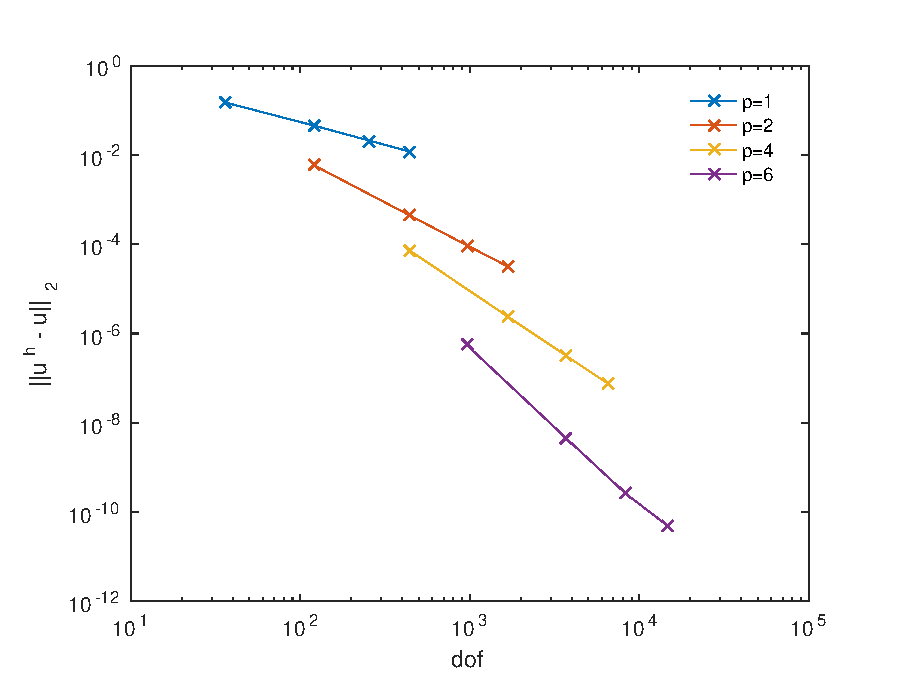
\includegraphics[width=0.45\textwidth]{conv_p2_reg.eps}
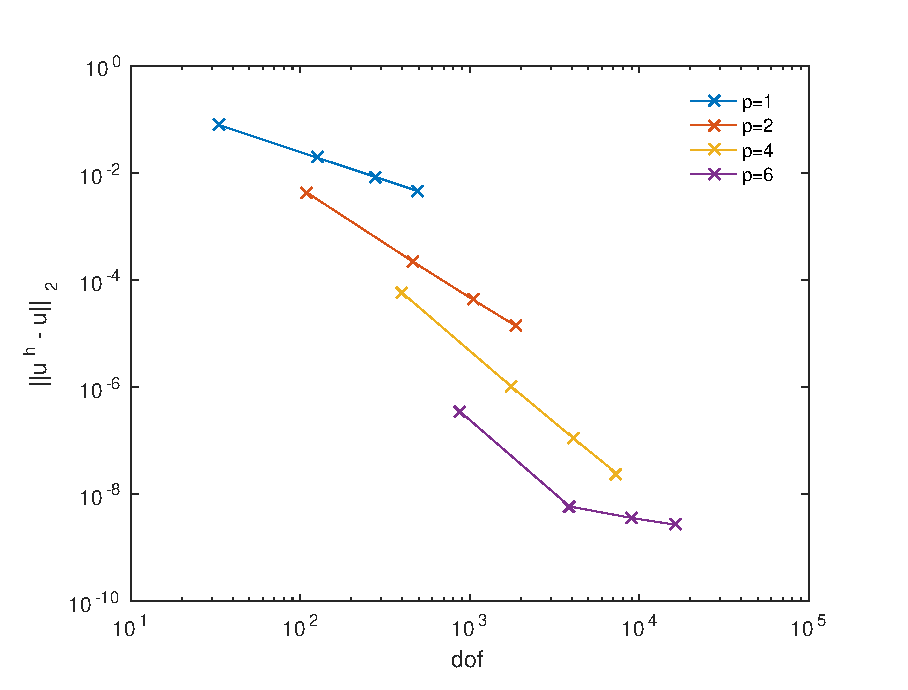
\includegraphics[width=0.45\textwidth]{conv_p2_ireg.eps}}
\caption{Convergence of for the case $p=2$ for polynomial order $1-5$, with various spatial refinement. Left: regular grid, right: irregular grid. }
\label{fig:convp2}
\end{figure}


\subsubsection*{$p\neq2$}

\subsection{Inverse problems}

\subsection{Model reduction}

\section{Stoke's flow with nonlinear rheology}

\subsection{Weakform}

\subsection{}

\end{document}
